% \begin{table*}[t]
\centering
\caption{$M_{miss}$ and $M_{remain}$ for \tool with the increases of entry nodes}
\label{tab:toolReductionAndMissing}
\resizebox{\textwidth}{!}{
\begin{tabular}{crrrrrrrrr}
\hline
%rowcolor[HTML]{C0C0C0} 
\textbf{Attack}        & \multicolumn{1}{c}{\textbf{1-$M_{miss}$}} & \multicolumn{1}{c}{\textbf{1-$M_{remain}$}} & \multicolumn{1}{c}{\textbf{1-$\# Edge$}} & \multicolumn{1}{c}{\textbf{2-$M_{miss}$}} & \multicolumn{1}{c}{\textbf{2-$M_{remain}$}} & \multicolumn{1}{c}{\textbf{2-$\# Edge$}} & \multicolumn{1}{c}{\textbf{3-$M_{miss}$}} & \multicolumn{1}{c}{\textbf{3-$M_{remain}$}} & \multicolumn{1}{c}{\textbf{3-$\# Edge$}} \\ \hline
Wget Executable      & 0.00                                                                      & 0.0413                                                                    & 15.00                                                                     & 0.00                                                                         & 0.1350                                                                   & 49                                                                        & 0.00                                                                      & 0.1460                                                                      & 53.00                                                                     \\ 
%rowcolor[HTML]{C0C0C0} 
Illegal Storage      & 0.17                                                                      & 0.0010                                                                    & 63.00                                                                     & 0.00                                                                         & 0.0011                                                                   & 67                                                                        & 0.00                                                                      & 0.0012                                                                      & 77.00                                                                     \\ 
Illegal Storage 2    & 0.00                                                                      & 0.0016                                                                    & 604.00                                                                    & 0.00                                                                         & 0.0016                                                                   & 607                                                                       & 0.00                                                                      & 0.0017                                                                      & 628.00                                                                    \\ 
%rowcolor[HTML]{C0C0C0} 
Hide File            & 0.08                                                                      & 0.0002                                                                    & 800.00                                                                    & 0.00                                                                         & 0.0002                                                                   & 805                                                                       & 0.00                                                                      & 0.0002                                                                      & 809.00                                                                    \\ 
Steal Information    & 0.00                                                                      & 0.0002                                                                    & 821.00                                                                    & 0.00                                                                         & 0.0003                                                                   & 854                                                                       & 0.00                                                                      & 0.0003                                                                      & 858.00                                                                    \\ 
%rowcolor[HTML]{C0C0C0} 
Backdoor Download    & 0.00                                                                      & 0.0009                                                                    & 55.00                                                                     & 0.00                                                                         & 0.0010                                                                   & 59                                                                        & 0.00                                                                      & 0.0021                                                                      & 129.00                                                                    \\ 
Annoying Server User & 0.00                                                                      & 0.0409                                                                    & 13.00                                                                     & 0.00                                                                         & 0.0660                                                                   & 21                                                                        & 0.00                                                                      & 0.0755                                                                      & 24.00                                                                     \\ 
%rowcolor[HTML]{C0C0C0} 
Shellshock           & 0.00                                                                      & 0.0719                                                                    & 33.00                                                                     & 0.00                                                                         & 0.1068                                                                   & 49                                                                        & 0.00                                                                      & 0.1089                                                                      & 50.00                                                                     \\ 
Dataleak             & 0.00                                                                      & 0.0742                                                                    & 17.00                                                                     & 0.00                                                                         & 0.1048                                                                   & 24                                                                        & 0.00                                                                      & 0.1135                                                                      & 26.00                                                                     \\ 
%rowcolor[HTML]{C0C0C0} 
VPN Filter            & 0.00                                                                      & 0.0287                                                                    & 19.00                                                                     & 0.00                                                                         & 0.0378                                                                   & 25                                                                        & 0.00                                                                      & 0.0408                                                                      & 27.00                                                                     \\ 
\textbf{AVG}         & 0.02                                                                      & 0.0261                                                                    & 244.00                                                                    & 0.00                                                                         & 0.0455                                                                   & 256                                                                       & 0.00                                                                      & 0.0490                                                                      & 268.10                                                                    \\ \hline
\end{tabular}
}
\end{table*}
% \input{tables/s&p/rq2random.tex}

\begin{figure}[t]
    \centering
    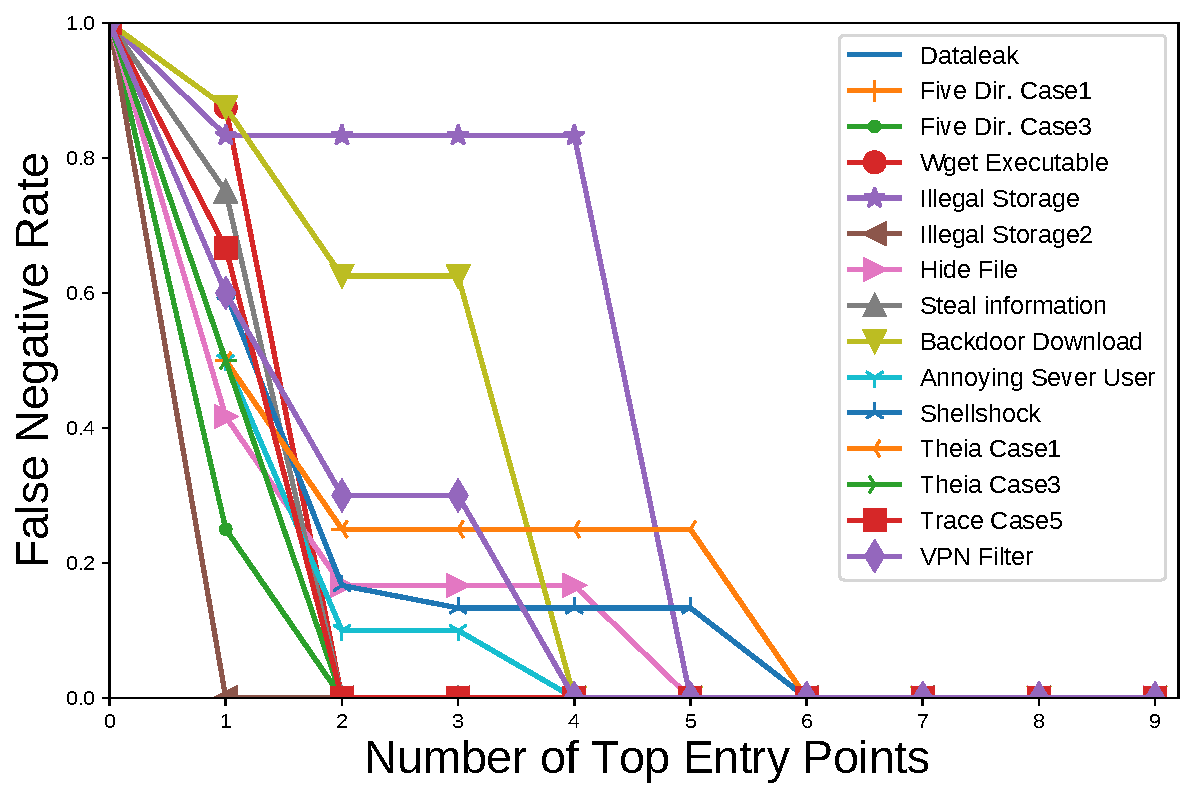
\includegraphics[width=\linewidth]{figs/falsenegative.pdf}
    \caption{False negative using different number of top-ranked entry nodes}
    \label{fig:rq2faslenegative}
\end{figure}
\begin{figure}[t]
    \centering
    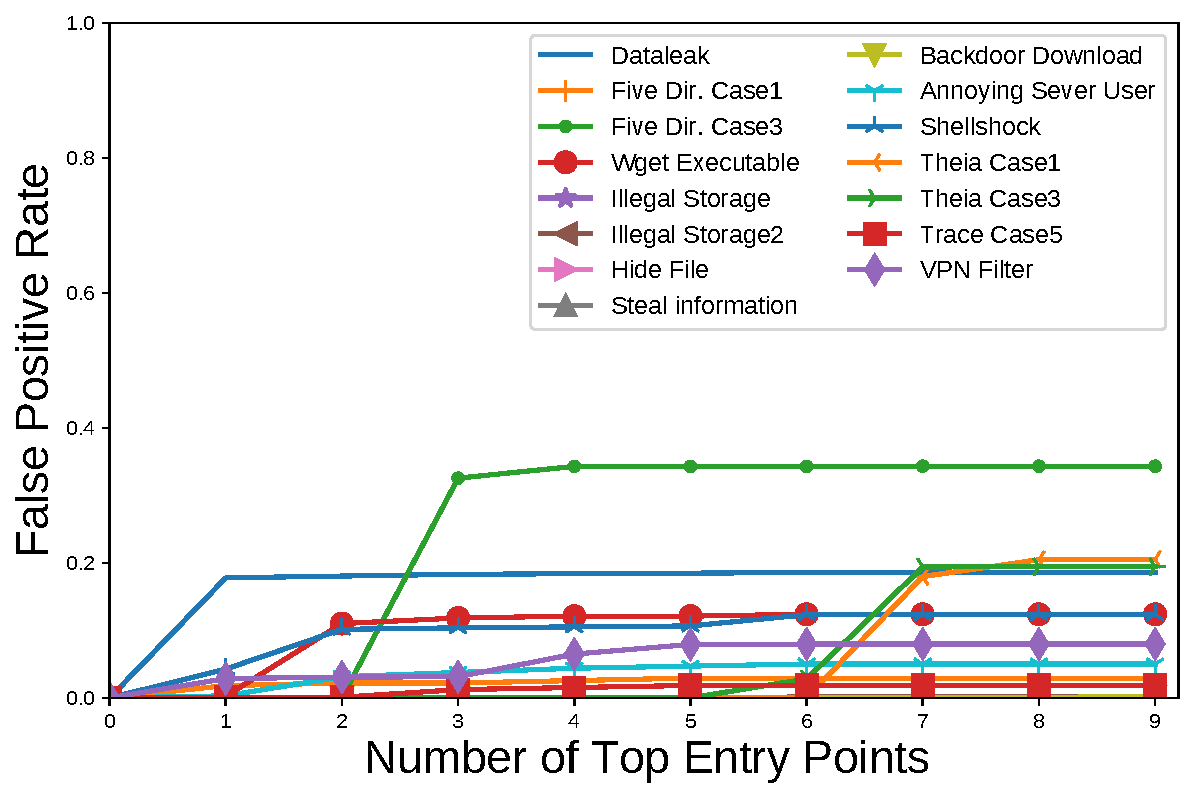
\includegraphics[width=\linewidth]{figs/falsepositive.pdf}
    \caption{False positive using different number of top-ranked entry nodes}
    \label{fig:rq2flasepositive}
\end{figure}

\subsection{RQ2: Selection of Entry Nodes}
\label{subsec:rq2}
% Given a dependency graph from a POI event, \tool chooses a number of top-ranked nodes to perform forward causality analysis, and remove the edges that cannot be found via the forward causality analysis.
Intuitively, the more entry nodes \tool uses to perform forward causality analysis, the less likely \tool will incorrectly filter out critical edges.
But using more entry nodes is likely to produce more false positives in the output graph.
%(\ie overlap of the forward dependency graph and the original backward dependency graph). 
To demonstrate the effectiveness of selecting the top-ranked entry nodes in revealing attack sequences, we show how the increase of the selected entry nodes impacts the effectiveness of \tool in terms of $FPR$ and $FNR$.
% As there are 3 types of system entities (\ie processes, files, and network connections) and hundreds or even thousands of entry nodes, 
\tool chooses the top-ranked entry nodes in each of three system-entity categories and perform forward causality analysis from the nodes in the order of decreasing dependency impacts.
% We evaluate the effectiveness of two mechanisms in selecting top-ranked entry nodes: one considers the types of system entities and the other does not.
% We measure the effectiveness of  selected the top-ranked entry nodes.

% we first compare \tool with a random approach that randomly selects entry nodes to perform forward causality analysis for filtering. 
% For \tool, we choose top 1, top 2, and top 3 entry nodes from the 3 types of system entities to perform the graph reduction. 
% For the random approach, we choose the 3, 6, and 9 entry nodes for fair comparison.




\eat{
\myparatight{Impacts on $M_{miss}$ and Edge Number}
\cref{fig:rq2missing} and \cref{fig:rq2edge} show the results of $M_{miss}$ and the edge number in the critical components.
As expected, when more entry nodes are used, $M_{miss}$ decreases while the edge number increases.
To reduce $M_{miss}$ to zero, $\sim50.0\%$ of the cases (8 attacks) use only two top-ranked nodes, and $73.3\%$ of the cases (11 attacks) use 4 top-ranked nodes.
We can also see that 6 entry nodes can cover all the attack entries for all the attack cases, and more entry nodes merely contribute to the increase of the irrelevant edges.
As shown in \cref{fig:rq2edge}, there is a sharp increase of the edge numbers when more than 6 entry nodes are used.
As such, when using \tool to investigate an attack, we can first select 2 top-ranked entry nodes, and include more entry nodes one by one until adding one more entry node will result in a sharp increase of the graph size.
The resulting graph typically will not miss any critical edge and still has a reasonably small size. }


\myparatight{Impacts on FPRs and FNRs}
\cref{fig:rq2faslenegative} and \cref{fig:rq2flasepositive} show the impacts of top entry nodes on $FPR$s and $FNR$s.
As expected, when more entry nodes are used, the $FNR$ decreases while the $FPR$ increases. 
We can notice that when the $FNR$ becomes zero  (using $2-6$ nodes in different attacks), if \tool continues to utilize more entry nodes to do the forward analysis, $FPR$ will increase significantly.
Based on this observation, we suggest that \tool stops choosing more entry nodes when including one more entry node for forward analysis will result in a significant increase of the critical component.


% This is because performing the forward causality analysis from more entry nodes will make the final graph overlap larger, which is likely to include more critical edges and more non-critical edges. 
% We can see that the decrease of $M_{miss}$ and more edges by using more top-ranked entry nodes in \cref{fig:rq2missing} and \cref{fig:rq2edge}.
% On average, the dependency graphs that preserve all critical edges contains only $158.73$ edges, which is significantly smaller than the original dependency graph.


\eat{
We further confirm that these 
Another finding is that the dependency impact of the node ranked at the third is about $70\%$ of the top 1 node's dependency impact.
Thus, alternatively, we can use $70\%$ of the top 1 node's dependency impact as the threshold to choose the top-ranked entry nodes for filtering.
}
